\documentclass[a4paper,12pt]{article}

\usepackage[T2A]{fontenc}
\usepackage[utf8]{inputenc}
\usepackage[serbianc]{babel}
\usepackage{amsmath,amssymb,amsthm}
\usepackage{graphicx}
\usepackage{array}
\usepackage{geometry}
\usepackage{hyperref}

\geometry{margin=2.5cm}

\newtheorem{definicija}{Definicija}
\newtheorem{lema}{Lema}
\newtheorem{teorema}{Teorema}

\title{Черч--Тјурингова теза и границе израчунљивости}
\author{Михајло Кончар}
\date{15. јануар 2026.}

\begin{document}

\maketitle
\tableofcontents
\newpage

\section{Увод}

Черч--Тјурингова теза представља један од најзначајнијих концепата
теоријске информатике и теорије израчунљивости. Она има за циљ да
формализује интуитивни појам алгоритма и да га повеже са строго
дефинисаним математичким моделима израчунавања.

Разумевање ове тезе омогућава јасно дефинисање граница онога што је
могуће израчунати помоћу рачунара.

\section{Историјски контекст}

Почетком XX века појавила се потреба за формалним описом појма
ефективног израчунавања. Алонзо Черч је 1936. године предложио
$\lambda$-рачун, док је Алан Тјуринг исте године увео концепт
Тјурингове машине.

Иако су ови модели настали из различитих теоријских приступа,
показано је да описују исту класу функција, што је довело до
формулисања Черч--Тјурингове тезе.

\section{Черч--Тјурингова теза}

\begin{definicija}
Черч--Тјурингова теза тврди да је свака функција која је интуитивно
израчунљива израчунљива помоћу Тјурингове машине.
\end{definicija}

Важно је нагласити да ова теза није теорема, јер интуитивни појам
алгоритма није формално дефинисан.

\section{Формални модели израчунавања}

\begin{lema}
Сваки алгоритам који се може описати коначним псеудокодом
може се симулирати Тјуринговом машином.
\end{lema}

\begin{teorema}
Тјурингове машине, $\lambda$-рачун и рекурзивне функције имају
еквивалентну израчунљиву моћ.
\end{teorema}

Ова еквиваленција представља снажан аргумент у прилог
Черч--Тјуринговој тези.

Најзначајнији формални модели су:

\begin{itemize}
    \item Тјурингова машина
    \item $\lambda$-рачун
    \item Рекурзивне функције
\end{itemize}

Основни кораци приликом анализе проблема су:

\begin{enumerate}
    \item Дефинисати проблем.
    \item Конструисати алгоритам.
    \item Анализирати сложеност алгоритма.
\end{enumerate}

\subsection{Границе израчунљивости}

Један од најпознатијих неразрешивих проблема је проблем заустављања.

\[
H(M,x)=
\begin{cases}
1, & \text{ако машина }M\text{ стане над улазом }x,\\
0, & \text{иначе.}
\end{cases}
\]

Показано је да не постоји алгоритам који може одлучити вредност
функције $H$ за све могуће програме и улазе.

Додатно важи

\[
\neg(p\land q)=\neg p\lor \neg q.
\]

\section{Поређење формалних модела израчунавања}

\begin{center}
\begin{tabular}{|p{3.2cm}|p{2.5cm}|p{5cm}|p{2.5cm}|}
\hline
\textbf{Модел} & \textbf{Аутор} & \textbf{Основна идеја} & \textbf{Израчунљива моћ}\\
\hline
Тјурингова машина & Алан Тјуринг & Апстрактан модел рачунања са бесконачном траком и главом за читање и писање & Еквивалентна\\
\hline
$\lambda$-рачун & Алонзо Черч & Формални систем заснован на примени и апстракцији функција & Еквивалентна\\
\hline
Рекурзивне функције & Клини, Гедел & Функције дефинисане почетним случајевима и рекурзивним корацима & Еквивалентна\\
\hline
\end{tabular}
\end{center}

\section{Илустрација}

\begin{figure}[h]
\centering
% Поставити слику у истом директоријуму
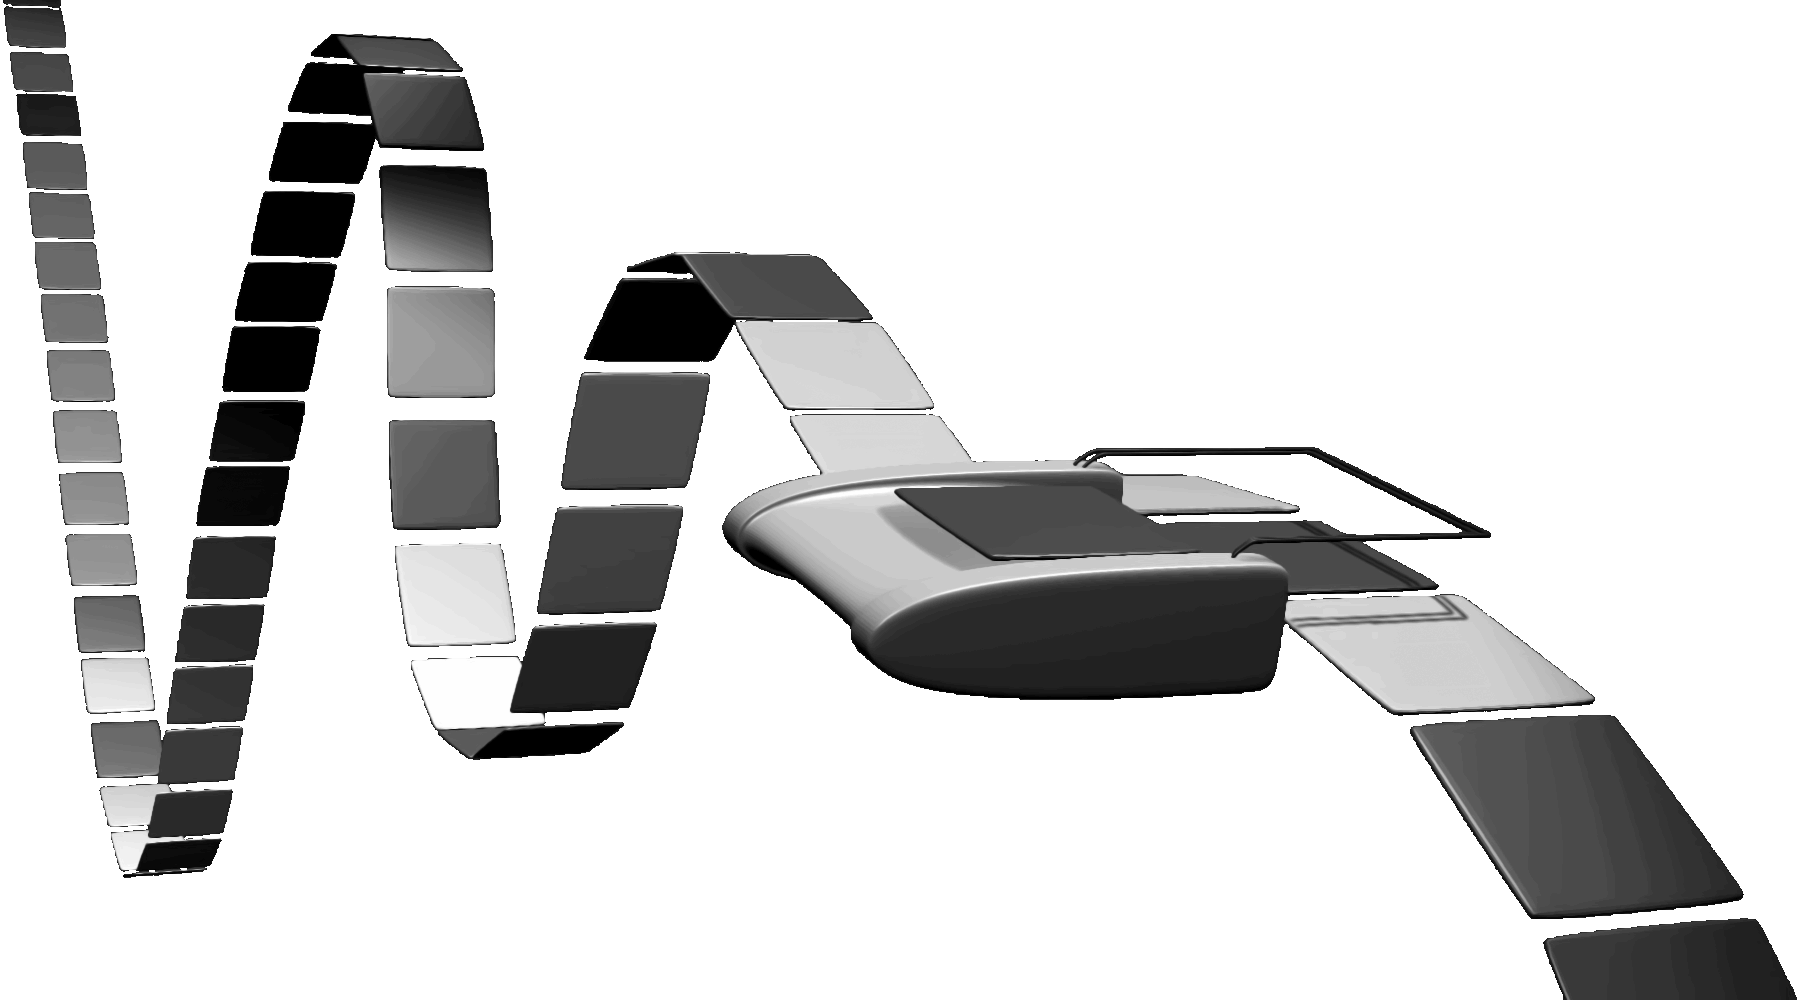
\includegraphics[width=0.55\textwidth]{slike/masina.png}
\caption{Шематски приказ Тјурингове машине.}
\end{figure}

\section{Закључак}

Черч--Тјурингова теза поставља јасне теоријске границе
израчунљивости и показује да постоје проблеми који се не могу
решити алгоритамски.

Ови резултати имају фундаментални значај за разумевање могућности
и ограничења рачунарских система.

\end{document}
